% !TeX root = main.tex
\chapter{Introduction \label{ch1-intro}}
	%1. state the general topic and give some background
		%a. It is about checking Flight Test Data. Within the FX-FTI department data is generated by aircraft. And right now it is also getting uploaded to the skystash platform to provide easier access to users instead of a long and tedious bureaucratic chain
Experimental Data is essential to confirm or nullify scientific theories. Motivated by sustainability the idea of Research Data Reuse culminated in the 2016 FAIR Guiding Principles \cite{wilkinson_fair_2016}. These principles stand for Findable, Accessible, Interoperable and Reusable data. This FAIR data usage by data creators in turn enables Open Data Access and Big Data within the scientific field. \cite{hodson_fair_2018} Within the German Aerospace Center (DLR) the Facility of Flight Experiments (FX) strives to fulfill FAIR principles for the Flight Test Data that gets generated by its fleet of 12 research aircraft. Within this work the ISTAR (In-flight Systems \& Technology Airborne Research) flight test aircraft, a Falcon 2000LX will be examined.
Since 2020 it is part of the DLR's research aicraft fleet, recording over 400 sensor parameters per flight. Within a FAIR context, the ISTAR-experimental data and metadata will be enriched and transformed into a FAIR-data format and then checked by a monitoring algorithm whose report also will result in a FAIR-data quality report. This standardized report format in turn allows creation of a standardized data quality visualization tool. This results in an architecture that is high in coherency but low in coupling improving maintainability and software quality.




The DLR's fleet of research aircraft is Europe's largest, consisting of 12 (as of 2023) different aircraft employed for atmospheric research up to testing operating limits and pushing the  aircraft operating envelope.

Within the department of Flight Test Instrumentation (FTI) within the DLR's Flight Experiments (FX) facility new methods are developed to reimagine data utilization.

Since the ISTAR is also core of the DLR's Digital Twin strategy its data gets uploaded to the newly developed skystash, a software architecture to distribute, analyze and visualize flight data. Utilizing these new possibilities, a new approach to fault detection is possible, postprocessing Flight Test Data and generating reports on data quality.

\paragraph{Topic}
%\section{What}
%Q:What is going to be examined within this thesis?
%E:

The data acquisitioning system (DAQ) plays a focal role in the generated data since it is the central data hub within the airplane. Making the DAQ as well as the sensor data the central point of this work.
In conjunction with the FAIR principles this work also focuses on reusability of the components of this work as well as interoperability with outside algorithms. Allowing the results of this work to be accessible by uploading them to the FAIR skystash data-platform and making condensing errors into tags and using conventions to catalyze digitalization to make the resulting data findable.
Hence, making it the goal of this thesis to examine the ISTAR DAQ in detail to detect sensor behavior anomalies and implement a clear infrastructure to fulfill FAIR principles.


%2. provide a review of the literature related to the topic
		%a. FMEA/data definitions
		%b. FAIR
		%c. Current skystash/digital twin
		%d. soil


Within this multidisciplinary work, previous efforts from the Fault-Mode Effect Analysis (FMEA) \cite{isermann_fault-diagnosis_2006} have been used in aircraft control systems and may be adapted for post-processing and detecting errors. Upon development and data handling, the FAIR (Findable, Accessible, Interoperable, Reusable) Guiding Principles \cite{wilkinson_fair_2016} are the state of the art for data operations, guaranteeing efficient and sustainable operations.
Other efforts include the development of the skystash, the aforementioned platform for developing the Digital Twin \cite{meyer_development_2020, arts_digital_2022} for the ISTAR to centralize data operations and distribution, digitizing the data and digitalizing the convoluted internal processes.
For organizing metadata in digitalized processes current developments are generally published within the Internet of Things (IoT), notable works are the Asset Administration Shell (AAS) \cite{bader_details_2020} and the work conducted at the WZL developing a higher level architecture of a SensOr Interfacing Language (SOIL) \cite{behrens_domain-specific_2021}.


	%3. define the terms and scope of the topic
		%a. Software needs to be developed to check data
		%b. Focus on integration and implementation of simple FMEA
The desired scope lies within developing a prototype for the Sensor Health Monitoring process. This includes designing and proposing interfaces for data and metadata along the data pipeline of generating data, merging metadata, checking data quality and finally generating a data quality report. Within the data quality check, a minimal running version of a FMEA shall be developed to test the system on its validity to check upon physical correlations.

	%4. outline the current situation
		%a. Data gets manually checked sometimes
		%b. Errors get detected late or never
		%c. Data in the skystash is unreliable
		%d. Experimental errors generate weird errors

The current data process contains various manual steps. This starts off at the Flight Data Parsing step which  consists of an FX-FTI employee manually converting the proprietary flight data via the proprietary IMC-Famos Software toward a Comma Separated Value-format (CSV) file format or  which then gets exported. The following steps then include uploading the data to a network drive and currently development is happening to also upload it to the skystash. After upload, there is no formalized data check happening. Any errors that are then detected mostly rely on coincidence to get detected.





	%5. evaluate the current situation (advantages/ disadvantages) and identify the gap
		%a. Disadvantage: no good error detection, no FAIR
		%b. Advantage: no negative reliability, hence illusion of reliable data (perhaps necessating investments of funds and time into sensors that are found to be unreliable)

This can lead to costly replications of experiments. In addition, FAIR principles are currently not fulfilled within the data lifecycle. While the current situation may have some disadvantages, some advantages of the current system could be a "don't ask, don't tell" philosophy. In this state a SHM could eventually uncover many previously unknown faults and thus necessitate investments of time and funds into reevaluation sensor hard- and software that are found to be unreliable.



To achieve this it is vital to increase the fault detection rate since sensor faults are frequently not detected). Commonly, a sensor- or system-failure may not be detected during a flight experiment but weeks after. This rescheduling within the aircrafts full timetable makes it even more economically important to implement a system to catch sensor faults and failures to avoid the need for an experiment to be reflown. A worst case scenario could be that a whole experiment needs to be replicated with the configuration needing to be recustomized and refitted which is a time- and funding intensive task.
Additionally, it is important to increase reaction time. Often errors are detected weeks after the flight is over. With a software detecting errors directly after sensor data is extracted from the aircraft errors may be detected on the same day. allowing a quicker reaction maybe repeating the experiment during the affixed timeslot.


%6. identify the importance of the proposed research
		%○ Costly mistakes/faults
		%○ Better overview
		%○ Quicker reaction time
		%○ Fulfillment FAIR (quick overview)
		%○ Safety critical errors may be reported



Research Introduction
	7. state the research problem/ questions
		a. Implementation of a FAIR SHM
	8. state the research aims and/or research objectives
		a. Finding of common data quality descriptors and definitions
		b. Find a fmea
		c. Implement the fmea into the skystash ecosystem
		d. validate
	9. state the hypotheses
		○ Proposal SHM
		○ Detect errors and report them
	10. outline the order of information in the thesis
		a. Descriptors
		b. Fmea
		c. Skystash, metadata
	11. outline the methodology
		i. Turbine model will be used for exploration and implementation of methods
		ii. FAIR
		iii. High coherency, low coupling








\paragraph{Motivation}
%Q: Why is this important?

It is then important to reduce manual overview of sensors. Currently, much manual postprocessing is needed to get an overview over the large datasets. Large datasets however are difficult to work with due to being too large for a single computer. Necessitating a server architecture for work with this size of data.
Another benefit of this work may be to reduce downtime of the Aircraft due to sensors. A diagnostic tool for detecting sensor behavior can facilitate the processes and allow a quicker follow up to detect sensor errors since currently system information is distributed and not clearly perceivable.

Safety critical errors may be detected earlier since the proposed routine has potential to go beyond the scope of commercially tested software that is generally employed within aircraft and generally rudimentary resulting from the desire to employ very stable software.
Once, a baseline routine is in place. It is then possible to build a foundation for a reliability index for sensors. This is vital for big data operations within digitalization and the skystash project. This should be able to implemented by plug and play into this works results. Allowing for quick implementation of custom data quality algorithms.

Another motivation for this work is the fulfillment of the FAIR (Findable, Accessible, Interoperable, Reusable) principles. FAIR principles are the new standard within the DLR for research data management. The use within operations however are far from the fulfillment. Documents containing descriptions of sensors and setups are distributed among multiple employees obstructing any efforts to comprehend the already complex aircraft system and its inherent generation of data.

The proposed work is then nothing short of essential, building a tool for detection and avoidance of sensor failures to mitigate risks associated with experimental setups since aircraft hours are expensive and the amount of sensors is vast.

\begin{figure}
    \centering
    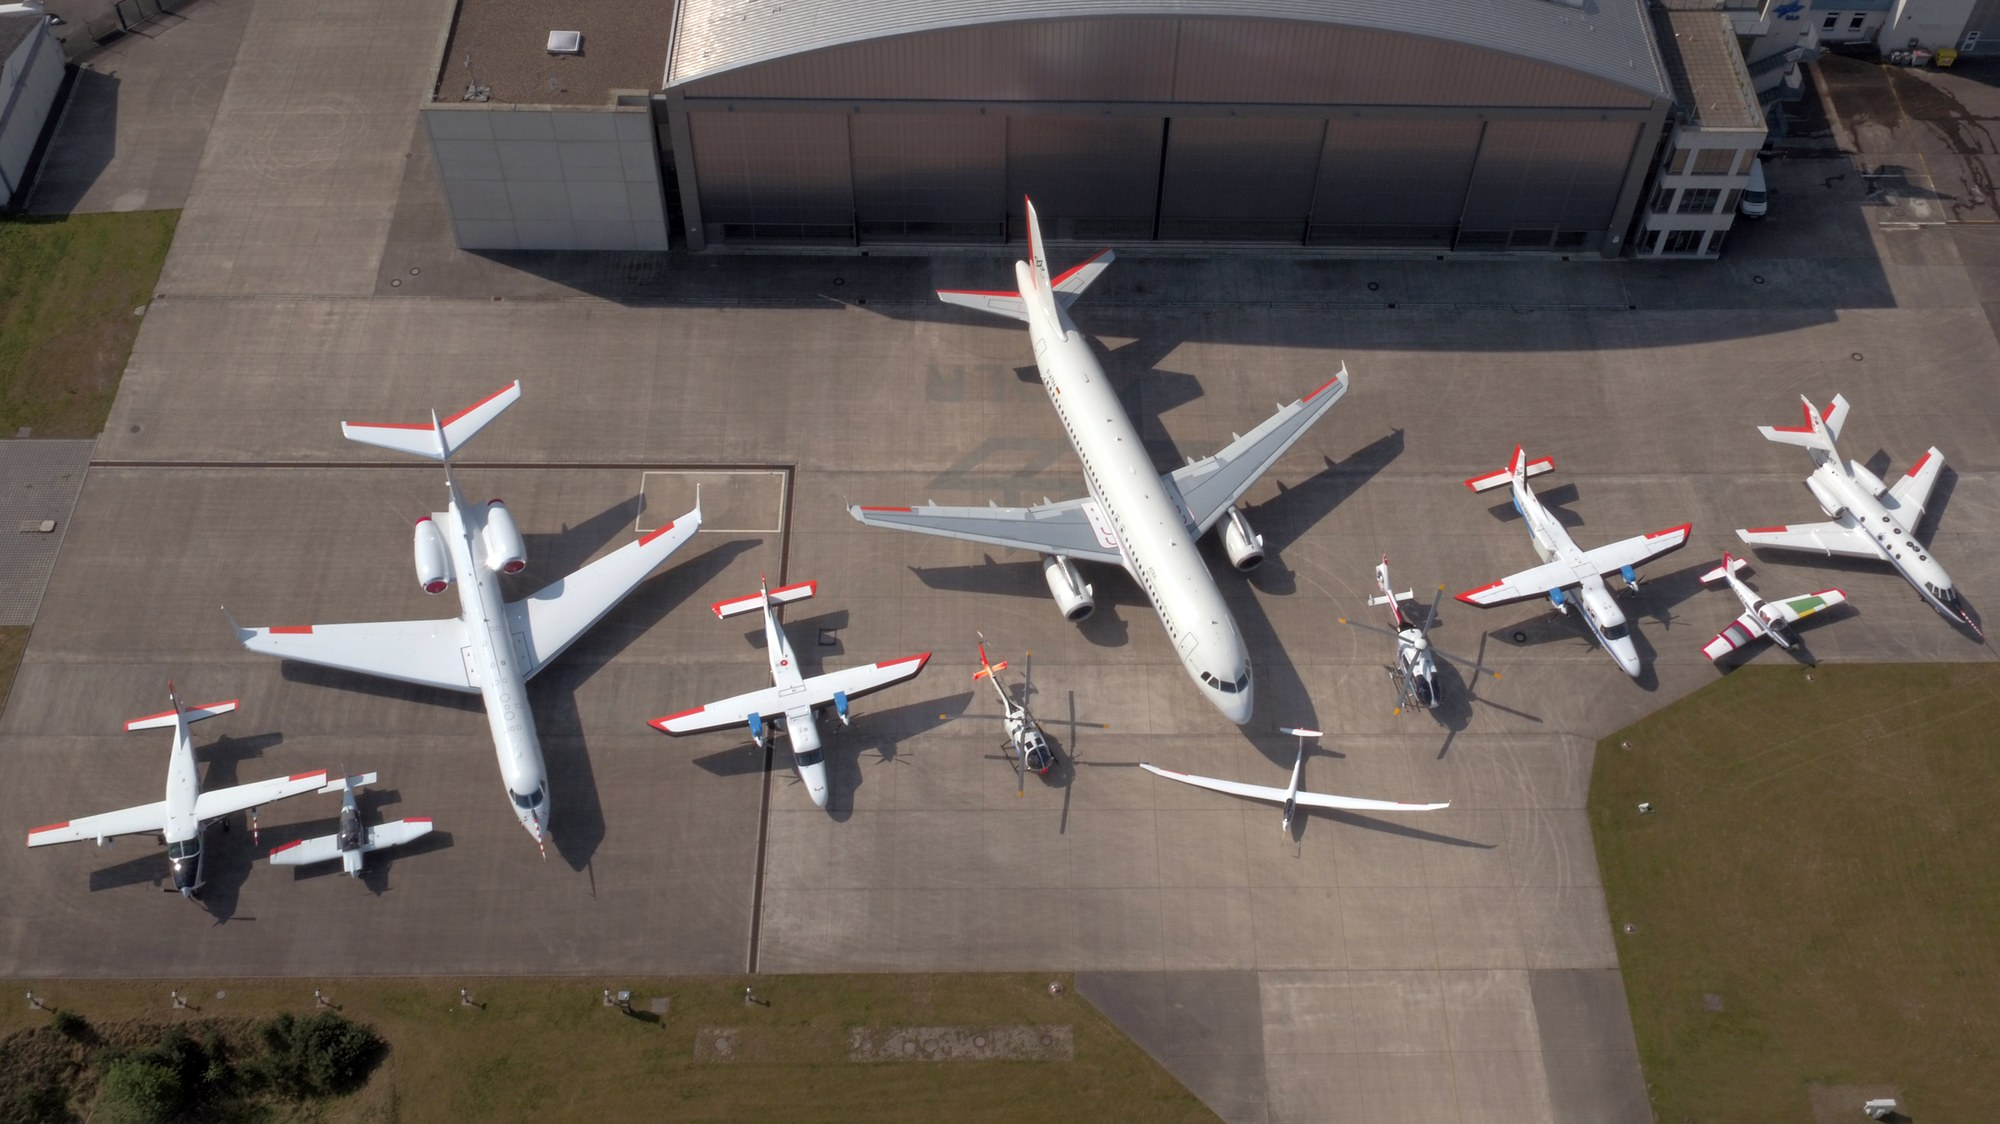
\includegraphics[width=0.7\textwidth]{dlr_fleet.jpeg}
    \caption{The DLR's research fleet \cite{dlr_dlr-fleet_2018}}
    \label{fig:dlr_fleet}
\end{figure}



\paragraph{State Research}
%Q: How to solve this rather extensive problem of SHM?
To now solve this extensive problem of SHM, it is possible to employ one of many existing methods in the field of Fault Detection and Mode Analysis (FMEA).

FMEA is a common problem in engineering disciplines and everywhere where systems become complex. %Literature is rich in this regard, so finding an appropriate solution should be a feasible undertaking
This problem also gets facilitated by the work that is already happening within the digital twin program within the DLR. A data space is already in development and is supplied with Flight Test Data which aids this work.
It is then necessary to allow clear software interfaces to facilitate future extensions and modes to allow reaching a quick overview over sensor errors.
FMEA is a rich field in which much energy has already been invested into similar problems. A new challenge arises from the implementation into a dynamic digital system also keeping in mind to remain open for new changes and addons.

%Q: whats the context on this work?

\paragraph{Context}
This work happens within the DLRs effort to digitize and digitalize research data and update its research data management strategy.
%Part of DigECat project for ISTAR digital twin
Within this project's scope, the development of skystash architecture is advanced to beyond prototypical level, allowing upload and distribution of research data by using the skystash cloud.
Within the scope of future work lies the expansion of metadata management on a larger scale, metadata frameworks already exists but challenges arise from indexing and providing a digital replica of long paper trails. Aircraft are highly complex systems that amass a great amount of paperwork since even its tiniest screws require a highly documented certification process.
%Further big data efforts also include data analytics allowing for easy scaling of this data base format
%For now, present work: work on prototypes of metadata management to represent sensor data. Calculations then can happen based on datasets with provided metadata without additional inputs.

Digitalization and the digital twin are the inherent adjuncts of this work. A database with data already exists. now it is time to structure metadata allowing for this work to happen dynamically. Building upon this, further metadata may be fed into the system allowing further analytics to be developed.


\paragraph{Summary}

This work will examine the sensor data of the ISTAR aircraft, examining various algorithms and methods for FMEA. Then developing a software that allows dynamic implementations of various FMEAs to generate a dynamic backend facilitating development and finally generating reports on data quality for the aircraft systems. FAIR principles are vital for future legibility and exchangeability of data and hence become a central part of this thesis facilitating future use of the results generated within this work.



% todo: von christina
% why?
% 1. actually detect data errors
% 2. promptly detect errors. manual diagnosis steps --> reduce downtime
% 3. increase quality of flight test data by marking errors to detect them

% todo: separate safety critical properties. Aircraft system: tested; DAQ-system not tested upon data quality and Fault Diagnosis system. FAult detections only shown in cockpit. not recorded for us.

% errors never or seldom detected